\documentclass[12pt,a4paper,ngerman,plainfootsepline,plainheadsepline]{scrreprt}
% Change "article" to "report" to get rid of page number on title page
\usepackage{amsmath,amsfonts,amsthm,amssymb}
\usepackage{setspace}
\usepackage{Tabbing}
\usepackage{lastpage}
\usepackage{cite}
\usepackage{tocbasic}
\usepackage[automark,						%Automatische Kopfzeile
						%headtopline,				%Linie über dem Seitenkopf
						%plainheadtopline,	%Plain, Linie über dem Seitenkopf
						headsepline,				%Linie zwischen Kopf und Textkörper
						%plainheadsepline,	%Plain, Linie zwischen Kopf und Textkörper
						footsepline,				%Linie zwischen Textkörper und Fuß
						plainfootsepline,   %Plain, Linie zwischen Textkörper und Fuß
						%footbotline,				%Linie unter dem Fuß
						%plainfootbotline   %Plain, Linie unter dem Fuß
						]{scrpage2}
\usepackage{graphicx,wrapfig}
%\usepackage[ansinew]{inputenc}
\usepackage{lmodern}
\usepackage{scrpage2}
\usepackage[utf8]{inputenc}
\usepackage[ngerman]{babel}
\usepackage{url}
\usepackage{fouriernc}
%\usepackage[scaled]{helvet}
\renewcommand*\familydefault{\sfdefault} %% Only if the base font of the document is to be sans serif
%\usepackage[T1]{fontenc}
% In case you need to adjust margins:
\topmargin=-0.45in      %
\evensidemargin=0in     %
\oddsidemargin=0in      %
\textwidth=6.5in        %
\textheight=9.0in       %
\headsep=0.25in         %
\setcounter{secnumdepth}{3}
\setcounter{tocdepth}{3}

% Homework Specific Information
\newcommand{\hmwkTitle}{Netzwerksicherheit}
\newcommand{\hmwkClass}{Handout}
\newcommand{\hmwkAuthorName}{Raphael Marques}

                                   %
\clearscrplain		
%Alte Plain-Formatierung entfernen
\clearscrheadfoot
\cehead{\hmwkClass}    % Chapter auf geraden Seiten (links) in Kopfzeile
\cohead{\hmwkClass}
\rehead{\includegraphics[width=25pt]{graphicszhaw.jpgg}}    % Logo auf geraden Seiten (rechts) in Kopfzeile
\rohead{
\includegraphics[width=25pt]{graphics/zhaw.jpg}}   % Logo auf ungeraden Seiten (links) in Kopfzeile
\lehead{\hmwkTitle}    % Section auf geraden Seiten (rechts) in Kopfzeile
\lohead{\hmwkTitle} 

\refoot{\hmwkAuthorName}    % Chapter auf geraden Seiten (links) in Kopfzeile
\rofoot{\hmwkAuthorName}
%\rofoot{Seite\ \thepage\ von\ \pageref{LastPage}}    % Chaper auf geraden Seiten (links) in Kopfzeile
%\refoot{Seite\ \thepage\ von\ \pageref{LastPage}}
\setheadsepline{0.4pt}   
\setfootsepline{0.4pt}                                  %
\pagestyle{scrheadings}
\automark[chapter]{chapter}
 % Seitenstil aktivieren
%\renewcommand{\chapterpagestyle}{scrheadings}
% This is used to trace down (pin point) problems
% in latexing a document:
%\tracingall


%%%%%%%%%%%%%%%%%%%%%%%%%%%%%%%%%%%%%%%%%%%%%%%%%%%%%%%%%%%%%
% Make title
%\title{\vspace{2in}\textmd{\textbf{\ \hmwkTitle}}\\\normalsize\vspace{0.1in}\large{\hmwkClass}\\\vspace{0.1in}\large{\textit{}}\vspace{3in}}

%\author{\textbf{\hmwkAuthorName}}
%\author{\textbf{Miro Ljubicic}\\ljubimir@students.zhaw.ch}
%%%%%%%%%%%%%%%%%%%%%%%%%%%%%%%%%%%%%%%%%%%%%%%%%%%%%%%%%%%%%
\begin{document}
\begin{spacing}{1.1}
%
%\maketitle
%\newpage
%% Uncomment the \tableofcontents and \newpage lines to get a Contents page
%% Uncomment the \setcounter line as well if you do NOT want subsections
%%       listed in Contents
%%\setcounter{tocdepth}{1}
%%\tableofcontents
%%\newpage
%
%% When problems are long, it may be desirable to put a \newpage or a
%% \clearpage before each homeworkProblem environment
%
%\clearpage
%\begin{normalsize}
%\setcounter{tocdepth}{2}
%\tableofcontents
%\end{normalsize}
\section*{Lagebericht Ausspähen}
\paragraph{Ausspähen} heisst, Daten mithilfe oder über IT zu erlangen, ohne dass das Ziel etwas davon erfährt. Ausspähen ist ein aktuelles Thema und wird im grossen Umfang durchgeführt. Durch die Möglichkeiten, grosse Datenmengen zu analysieren (Stichwort BigData), ist es umso wertvoller, möglichst viel Daten zu erlangen.  Der Lagebericht ausspähen befasst sich mit der Definition von Ausspähen und stellt eine Übersicht über die aktuellen Arten der Spionage Bereit, welche in der Grafik am ende dieses Handouts ersichtlich sind. Folgendermassen werden in dem Lagebericht die Arten von Ausspähen kategorisiert:

\textbf{Aggressivität:} Man unterscheidet zwischen Footprinting, Vulnerability Scanning und Penetration Testing. Während Footprinting generelle Daten eines Ziels sammelt, und diese korreliert, sucht der Vulnerability Scan spezifisch nach Schwachstellen bei dem Ziel. Der Penetration Test versucht, diese Schwachstellen zu missbrauchen , Zugang auf das System zu erlangen und möglichst viel "'Schaden"' anzurichten.
 
\textbf{Ziel:} Ziele von Aussähen können natürliche Personen sein, oder die IT Infrastruktur selber. Letztere ist wichtig, für zusätzliche Angriffe auf eine natürliche Person.
 
\textbf{Aktiv/Passiv:} Eine wichtige Unterscheidung bei Ausspähen, ist der Kontakt mit dem Ziel. Bei aktivem Ausspähen wird auf irgendeinem Weg mit dem Ziel interagiert, während bei passivem Ausspähen kein Kontakt mit dem Ziel herrscht, sondern nur Informationen auf "'neutralen"' Plattformen gesammelt werden. 

Bei anschliessender Grafik sieht man eine Übersicht verschiedener Arten von Ausspähen, kategorisiert in obenstehende Definitionen:

\begin{figure}[h]
\centering
\vspace{-0.3cm}
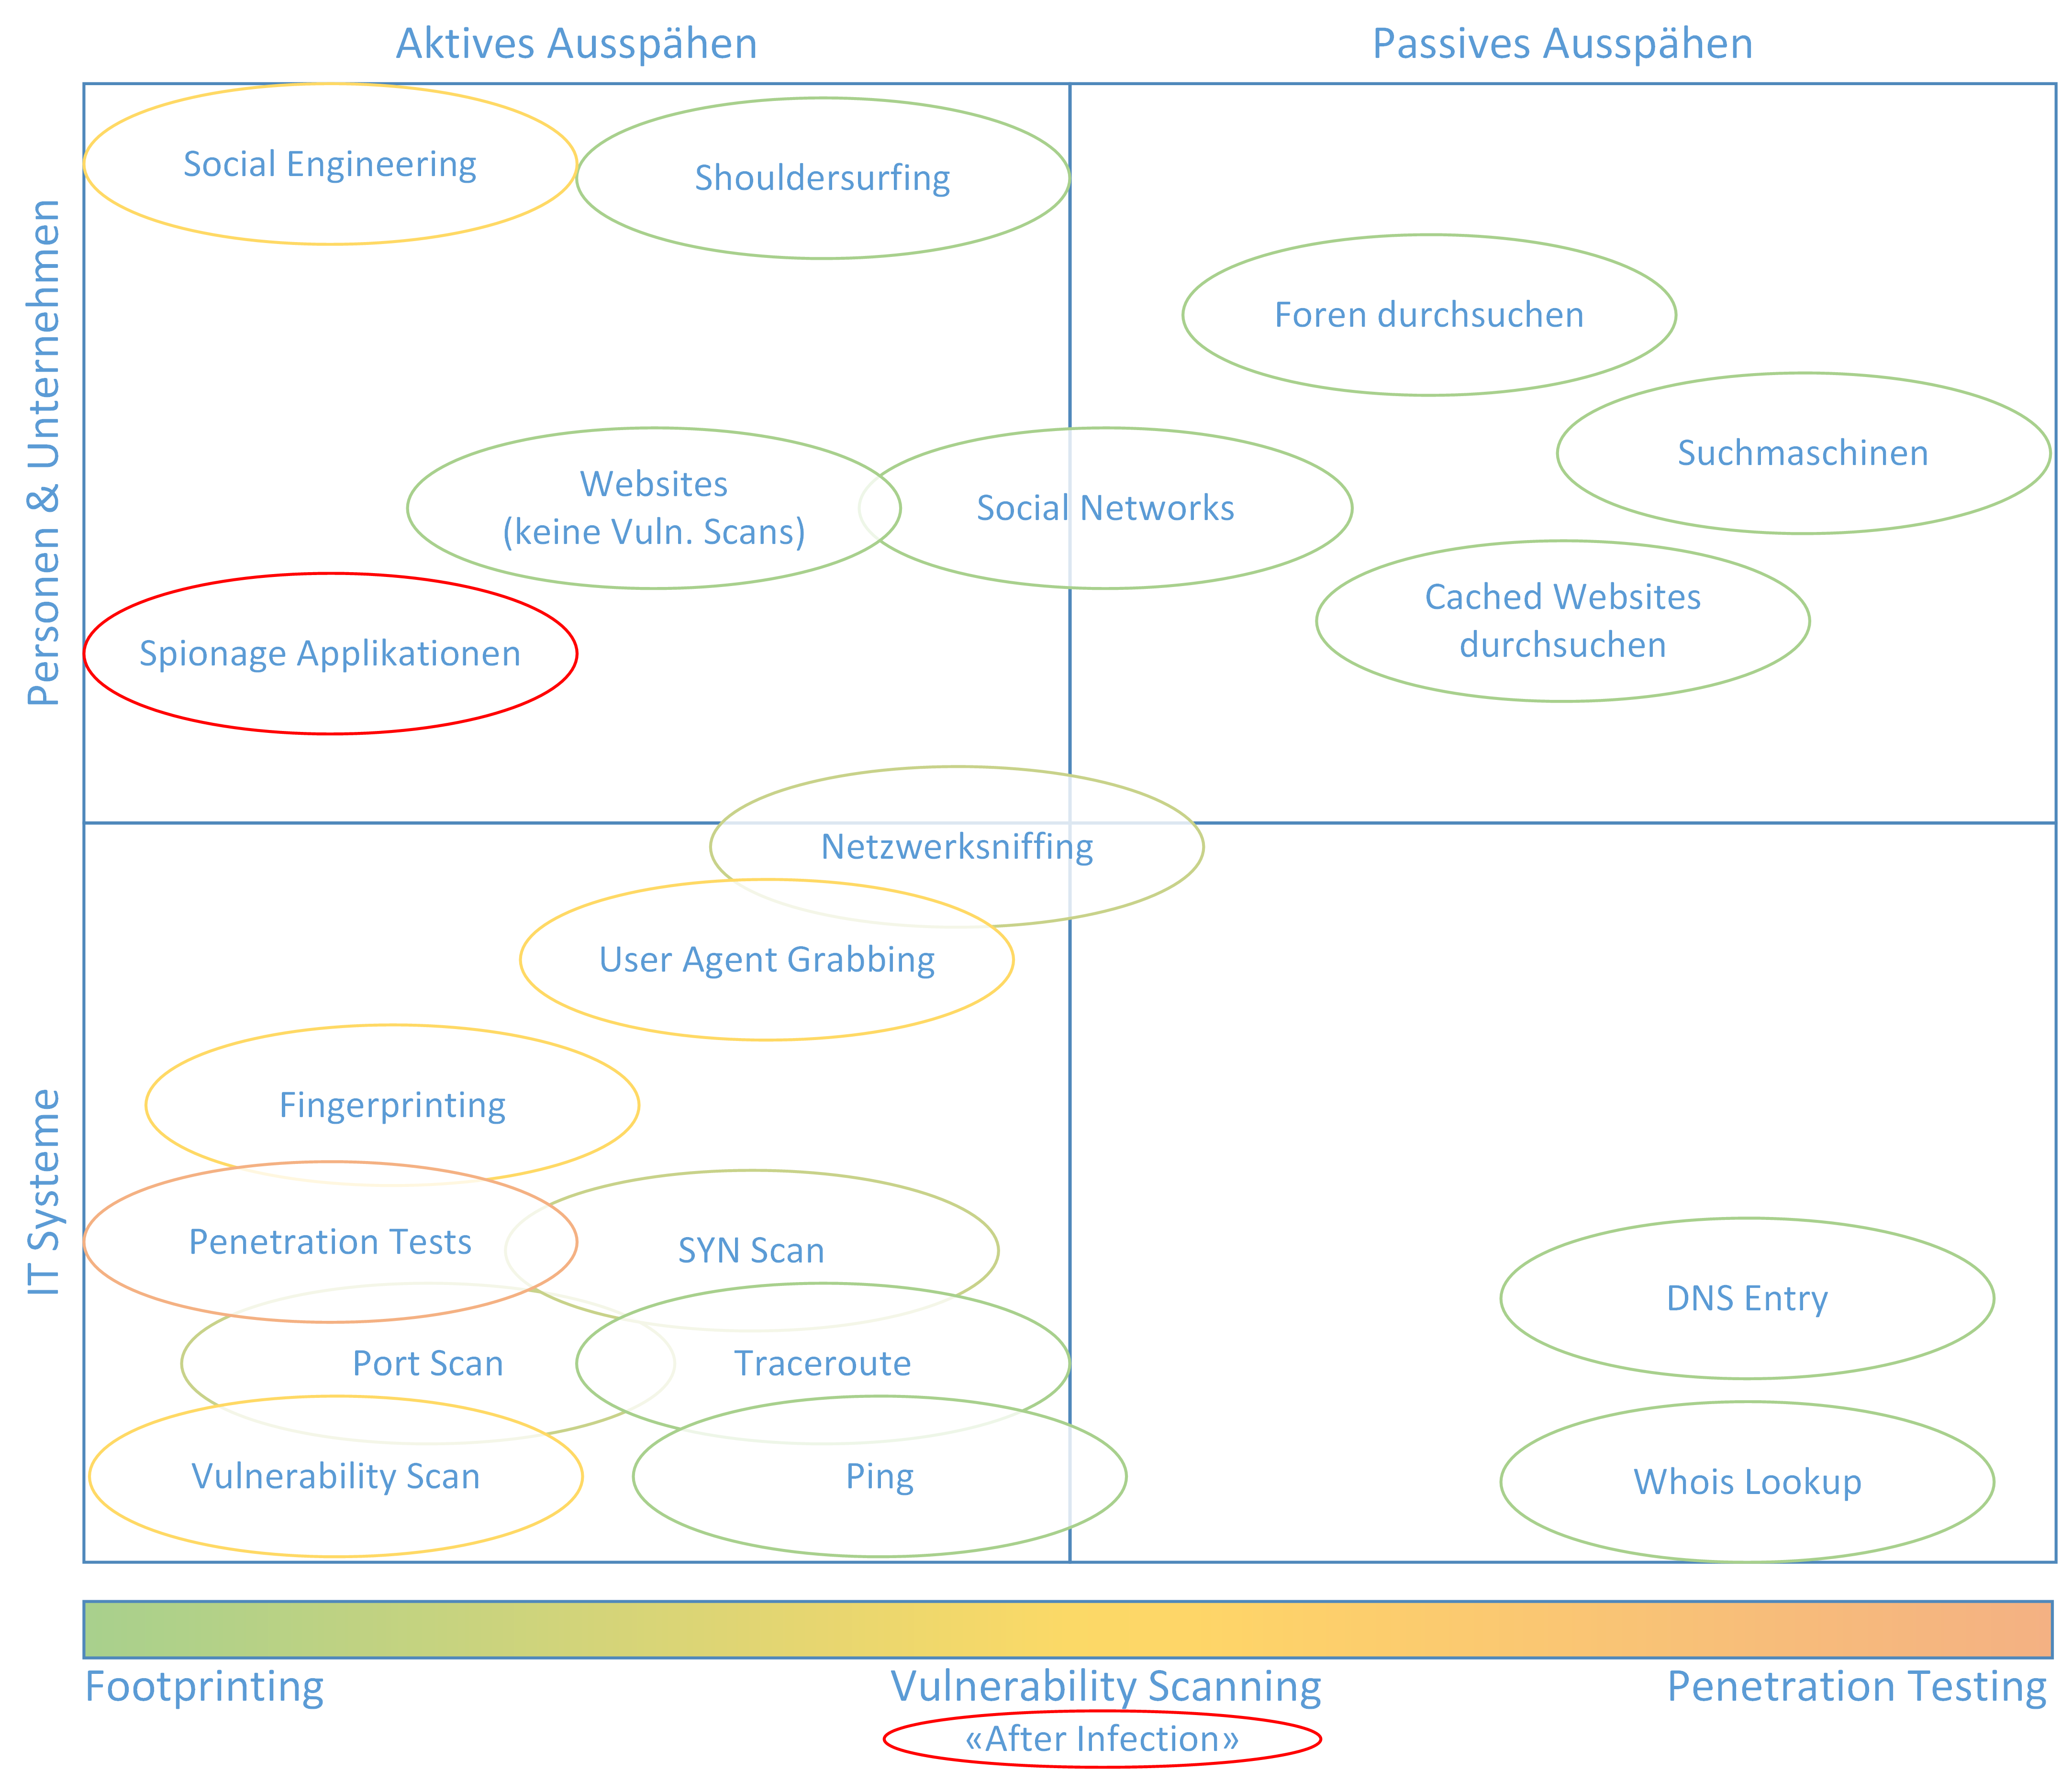
\includegraphics[width=0.8\linewidth]{../Graphics/uebersichtsmatrix.png}
\label{fig:itilv}
\vspace{-2.1
cm}
\end{figure}



%\input{subdoc/Glossar}
%\input{subdoc/Einleitung}
%\input{subdoc/Grundlagen}
%\input{subdoc/ISO_IEC_20000}
%\input{subdoc/Umsetzung_Praxis}
%\input{subdoc/Prozessbeispiel_Incident}
%\input{subdoc/Weiterer_Ausblick}
%\input{subdoc/Fazit}
%\input{subdoc/Anhang_A}
%\listoffigures
%\nocite{*} 
%\bibliography{bib/bib1}{}
%\bibliographystyle{plain}
%%\bibliographystyle{alphadin}
%%\bibliographystyle{plain}
\end{spacing}
\end{document}